\subsection{RELATION BETWEEN TWO ROOTS}

Recall that we assume from now on that k = R. (We leave to the reader the task of extending the definitions and results to the general case, by using the method indicated in Remark 2 of no. 1.)

Throughout the following, R denotes a root system in a vector space V; and V is equipped with a scalar product \((x,y)\mapsto(x|y)\) invariant under W(R), cf.~Prop. 3.

Let \(\alpha, \beta \in \mathbb{R}\) . By formula (7) of no. 1,

\[
n (\alpha , \beta) n (\beta , \alpha) = 4 \cos^ {2} (\widehat {\alpha , \beta}) \leqslant 4.\tag{10}
\]

Thus, the integer \(n(\alpha,\beta)n(\beta,\alpha)\) must take one of the values 0, 1, 2, 3, 4. In view of Chap. V, § 2, no. 5, Cor. of Prop. 6, and of the footnote on the page of Chap. V, § 4, no. 8, we see that the only possibilities are the following, up to interchanging \(\alpha\) and \(\beta\) :

\[
1) \quad n (\alpha , \beta) = n (\beta , \alpha) = 0; \quad \widehat {(\alpha , \beta)} = \frac {\pi}{2}; \quad s _ {\alpha} s _ {\beta} \text {of order} 2;
\]

\[
2) \quad n (\alpha , \beta) = n (\beta , \alpha) = 1; \quad (\alpha , \beta) = \frac {\pi}{3}; \quad s _ {\alpha} s _ {\beta} \text {   of   order   } 3;
\]

\[
\parallel \alpha \parallel = \parallel \beta \parallel ;
\]

\[
3) \quad n (\alpha , \beta) = n (\beta , \alpha) = - 1;
\]

\[
\widehat {(\alpha , \beta)} = \frac {2 \pi}{3};
\]

\[
s _ {\alpha} s _ {\beta} \text {of order 3};
\]

\[
\| \alpha \| = \| \beta \|;
\]

\[
4) \quad n (\alpha , \beta) = 1, n (\beta , \alpha) = 2; \qquad \widehat {(\alpha , \beta)} = \frac {\pi}{4};
\]

\[
s _ {\alpha} s _ {\beta} \text {   of   order   4;   }
\]

\[
\parallel \beta \parallel = \sqrt {2} \parallel \alpha \parallel ;
\]

\[
5) \quad n (\alpha , \beta) = - 1, n (\beta , \alpha) = - 2;
\]

\[
\widehat {(\alpha , \beta)} = \frac {3 \pi}{4};
\]

\[
s _ {\alpha} s _ {\beta} \text {   of   order   4;   }
\]

\[
\parallel \beta \parallel = \sqrt {2} \parallel \alpha \parallel ;
\]

\[
6) \quad n (\alpha , \beta) = 1, n (\beta , \alpha) = 3;
\]

\[
\widehat {(\alpha , \beta)} = \frac {\pi}{6};
\]

\[
s _ {\alpha} s _ {\beta} \text {   of   order   } 6;
\]

\[
\parallel \beta \parallel = \sqrt {3} \parallel \alpha \parallel ;
\]

\[
7) \quad n (\alpha , \beta) = - 1, n (\beta , \alpha) = - 3;
\]

\[
\widehat {(\alpha , \beta)} = \frac {5 \pi}{6};
\]

\[
s _ {\alpha} s _ {\beta} \text {   of   order   6;   }
\]

\[
\parallel \beta \parallel = \sqrt {3} \parallel \alpha \parallel ;
\]

\begin{enumerate}
\def\labelenumi{\arabic{enumi})}
\setcounter{enumi}{7}
\item
  \(n(\alpha, \beta) = n(\beta, \alpha) = 2; \quad \alpha = \beta;\)
\item
  \(n(\alpha, \beta) = n(\beta, \alpha) = -2; \quad \alpha = -\beta;\)
\item
  \(n(\alpha, \beta) = 1\) , \(n(\beta, \alpha) = 4\) ; \(\beta = 2\alpha\) ;
\item
  \(n(\alpha, \beta) = -1\) , \(n(\beta, \alpha) = -4\) ; \(\beta = -2\alpha\) .
\end{enumerate}

In particular:

PROPOSITION 8. (i) If two roots are proportional, the factor of proportionality can only be \(\pm 1, \pm \frac{1}{2}, \pm 2\) .

\begin{enumerate}
\def\labelenumi{(\roman{enumi})}
\setcounter{enumi}{1}
\tightlist
\item
  If \(\alpha\) and \(\beta\) are two non-proportional roots, and if \(\| \alpha \| \leqslant \| \beta \|\) , then \(n(\alpha, \beta)\) takes one of the values \(0, 1, -1\) .
\end{enumerate}

If a root \(\alpha \in \mathbb{R}\) is such that \(\frac{1}{2}\alpha \notin \mathbb{R}\) , then \(\alpha\) is called an indivisible root.

THEOREM 1. Let \(\alpha, \beta\) be two roots.

\begin{enumerate}
\def\labelenumi{(\roman{enumi})}
\item
  If \(n(\alpha, \beta) > 0\) , \(\alpha - \beta\) is a root unless \(\alpha = \beta\) .
\item
  If \(n(\alpha, \beta) < 0\) , \(\alpha + \beta\) is a root unless \(\alpha = -\beta\) .
\end{enumerate}

If \(n(\alpha, \beta) > 0\) , the possibilities, by the list above, are the following:

\begin{enumerate}
\def\labelenumi{\arabic{enumi})}
\item
  \(n(\alpha, \beta) = 1\) ; then \(\alpha - \beta - s_{\beta}(\alpha) \in \mathbb{R}\) ;
\item
  \(n(\beta, \alpha) = 1\) ; then \(\beta - \alpha = s_{\alpha}(\beta) \in \mathbb{R}\) , so \(\alpha - \beta \in \mathbb{R}\) ;
\item
  \(\beta = \alpha\) .
\end{enumerate}

This proves (i), and (ii) follows by changing \(\beta\) to \(-\beta\) .

COROLLARY. Let \(\alpha\) and \(\beta\) be two roots.

\begin{enumerate}
\def\labelenumi{(\roman{enumi})}
\item
  If \((\alpha |\beta) > 0\) , \(\alpha - \beta\) is a root unless \(\alpha = \beta\) .
\item
  If \((\alpha |\beta) < 0\) , \(\alpha + \beta\) is a root unless \(\alpha = -\beta\) .
\item
  If \(\alpha - \beta \notin R \cup \{0\}\) and \(\alpha + \beta \notin R \cup \{0\}\) , then \((\alpha | \beta) = 0\) .
\end{enumerate}

Assertions (i) and (ii) follow from Th. 1 and formula (7) of no. 1. Assertion (iii) follows from (i) and (ii).

It is possible that \(\alpha + \beta \in \mathbb{R}\) , \((\alpha|\beta) = 0\) (cf.~Plate X, System \(B_{2}\)). When \(\alpha - \beta \notin \mathbb{R} \cup \{0\}\) and \(\alpha + \beta \notin \mathbb{R} \cup \{0\}\) , \(\alpha\) and \(\beta\) are said to be strongly orthogonal.

PROPOSITION 9. Let \(\alpha\) and \(\beta\) be two non-proportional roots.

\begin{enumerate}
\def\labelenumi{(\roman{enumi})}
\item
  The set I of integers \(j\) such that \(\beta + j\alpha\) is a root is an interval \([-q, p]\) in \(\mathbf{Z}\) containing 0.
\item
  Let \(S\) be the set of \(\beta + j\alpha\) for \(j \in I\) . Then,
\end{enumerate}

\[
s _ {\alpha} (S) = S \text { and } s _ {\alpha} (\beta + p \alpha) = \beta - q \alpha .
\]

\begin{enumerate}
\def\labelenumi{(\roman{enumi})}
\setcounter{enumi}{2}
\tightlist
\item
  \(p - q = -n(\beta, \alpha)\) .
\end{enumerate}

Clearly, \(0 \in I\) . Let \(p\) (resp. \(-q\) ) be the largest (resp. smallest) element of \(I\) . If not all the integers in \([-q, p]\) belong to \(I\) , there exist two integers \(r, s\) in \([-q, p]\) with the following properties: \(s > r + 1\) , \(s \in I\) , \(r \in I\) , \(r + k \notin I\) for \(1 \leqslant k \leqslant s - r - 1\) . With the notation of the Cor. of Th. 1, \((\alpha|\beta + s\alpha) \leqslant 0\) , \((\alpha|\beta + r\alpha) \geqslant 0\) , which is absurd because

\[
(\alpha | \beta + s \alpha) \leqslant 0 > (\alpha | \beta + r \alpha).
\]

This proves (i).

We have \(s_{\alpha}(\beta + j\alpha) = \beta - n(\beta, \alpha)\alpha - j\alpha = \beta + j'\alpha\) with \(j' = -j - n(\beta, \alpha)\) . Thus \(s_{\alpha}(S) \subseteq S\) and consequently \(s_{\alpha}(S) = S\) . Now \(j \mapsto -j - n(\beta, \alpha)\) is a decreasing bijection from I to I. It follows that, \(j' = -q\) when \(j = p\) , so that \(-q = -p - n(\beta, \alpha)\) . This proves (ii) and (iii).

The set S is called the \(\alpha\) -chain of roots defined by \(\beta\) , \(\beta - q\alpha\) is its origin, \(\beta + p\alpha\) is its end, and \(p + q\) is its length.

COROLLARY. Let S be an \(\alpha\) -chain of roots, and \(\gamma\) the origin of S. The length of S is \(-n(\gamma,\alpha)\) ; it is equal to 0, 1, 2 or 3.

The first assertion follows from Prop. 9, (iii), applied to \(\beta = \gamma\) , and using the fact that \(q = 0\) .

On the other hand, since \(\gamma\) is not proportional to \(\alpha\) , the list given at the beginning of this no. shows that \(|n(\gamma,\alpha)|\leqslant3\) , hence the corollary.

Remark. We retain the notation above. Then:

\begin{enumerate}
\def\labelenumi{\arabic{enumi})}
\item
  If the length of S is 0, then \((\alpha |\gamma) = 0\) .
\item
  If the length of \(S\) is 1, then \(n(\gamma, \alpha) = -1\) , and there are three cases:
\end{enumerate}

\[
n (\alpha , \gamma) = - 1, \quad (\alpha | \alpha) = (\gamma | \gamma), \quad (\alpha | \gamma) = - \frac {1}{2} (\alpha | \alpha), \quad \widehat {(\alpha , \gamma)} = \frac {2 \pi}{3}
\]

\[
n (\alpha , \gamma) = - 2, \quad (\alpha | \alpha) = 2 (\gamma | \gamma), \quad (\alpha | \gamma) = - \frac {1}{2} (\alpha | \alpha), \quad \widehat {(\alpha , \gamma)} = \frac {3 \pi}{4}
\]

\[
n (\alpha , \gamma) = - 3, \quad (\alpha | \alpha) = 3 (\gamma | \gamma), \quad (\alpha | \gamma) = - \frac {1}{2} (\alpha | \alpha), \quad (\widehat {\alpha , \gamma}) = \frac {5 \pi}{6}
\]

\pandocbounded{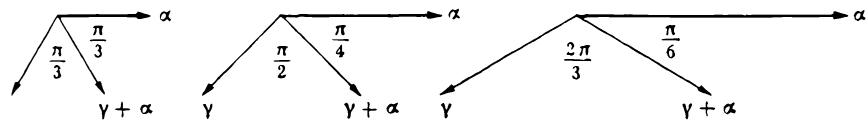
\includegraphics[keepaspectratio]{images/part001_d4d2d336.jpg}}

\begin{enumerate}
\def\labelenumi{\arabic{enumi})}
\setcounter{enumi}{2}
\tightlist
\item
  If the length of \(S\) is 2, then \(n(\gamma, \alpha) = -2\) , so
\end{enumerate}

\[
n (\alpha , \gamma) = - 1, (\alpha | \alpha) = \frac {1}{2} (\gamma | \gamma), (\alpha | \gamma) = - (\alpha | \alpha), \widehat {(\alpha , \gamma)} = \frac {3 \pi}{4}.
\]

\pandocbounded{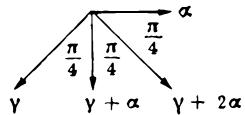
\includegraphics[keepaspectratio]{images/part001_f07fa75a.jpg}}

\begin{enumerate}
\def\labelenumi{\arabic{enumi})}
\setcounter{enumi}{3}
\tightlist
\item
  If the length of \(S\) is 3, then \(n(\gamma, \alpha) = -3\) , so
\end{enumerate}

\[
n (\alpha , \gamma) = - 1, (\alpha | \alpha) = \frac {1}{3} (\gamma | \gamma), (\alpha | \gamma) = - \frac {3}{2} (\alpha | \alpha), (\widehat {\alpha , \gamma}) = \frac {5 \pi}{6}.
\]

\pandocbounded{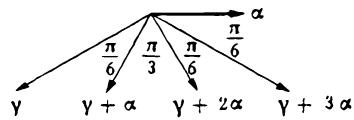
\includegraphics[keepaspectratio]{images/part001_9d247bec.jpg}}

We shall see (Plate X, Systems \(A_{2}, B_{2}, G_{2}\) ) that all these cases are actually realised.

PROPOSITION 10. Let \(\alpha, \beta\) be two non-proportional roots such that \(\beta + \alpha\) is a root. Let \(p, q\) be the integers in Prop. 9. Then

\[
\frac {(\beta + \alpha | \beta + \alpha)}{(\beta | \beta)} = \frac {q + 1}{p}.
\]

Let \(S\) be the \(\alpha\) -chain defined by \(\beta\) , \(\gamma\) its origin; its length \(l\) is \(\geqslant 1\) since \(\beta + \alpha\) is a root. The following cases are possible:

\begin{enumerate}
\def\labelenumi{\arabic{enumi})}
\item
  \(l = 1\) ; then \(\beta = \gamma, q = 0, p = 1, (\beta + \alpha | \beta + \alpha) = (\beta | \beta)\) .
\item
  \(l = 2\) , \(\beta = \gamma\) ; then \(q = 0\) , \(p = 2\) , \((\beta + \alpha|\beta + \alpha) = \frac{1}{2} (\beta|\beta)\) .
\item
  \(l = 2, \beta = \gamma + \alpha\) ; then \(q = 1, p = 1, (\beta + \alpha|\beta + \alpha) = 2(\beta|\beta)\) .
\item
  \(l = 3, \beta = \gamma\) ; then \(q = 0, p = 3, (\beta + \alpha | \beta + \alpha) = \frac{1}{3} (\beta | \beta)\) .
\item
  \(l = 3, \beta = \gamma + \alpha\) ; then \(q = 1, p = 2, (\beta + \alpha|\beta + \alpha) = (\beta|\beta)\) .
\item
  \(l = 3\) , \(\beta = \gamma + 2\alpha\) ; then \(q = 2, p = 1\) , \((\beta + \alpha|\beta + \alpha) = 3(\beta|\beta)\) .
\end{enumerate}

In each case, the formula to be proved is satisfied.

PROPOSITION 11. Assume that R is irreducible. Let \(\alpha\) and \(\beta\) be two roots such that \(\| \alpha \| = \| \beta \|\) . There exists \(g \in \mathrm{W}(\mathbb{R})\) such that \(g(\alpha) = \beta\) .

The transforms of \(\alpha\) by W(R) generate V (no. 2, Cor. of Prop. 5). Hence there exists \(g \in \mathrm{W}(\mathbb{R})\) such that \((g(\alpha)|\beta) \neq 0\) . We assume from now on that \((\alpha|\beta) \neq 0\) . By formula (9) of no. 1, \(n(\alpha, \beta) = n(\beta, \alpha)\) . Replacing \(\beta\) if necessary by \(s_{\beta}(\beta) = -\beta\) , we can assume that \(n(\alpha, \beta) > 0\) . Then, by the list at the beginning of no. 3, either \(\alpha = \beta\) (in which case the proposition is clear), or \(n(\alpha, \beta) = n(\beta, \alpha) = 1\) ; in that case

\[
s _ {\alpha} s _ {\beta} s _ {\alpha} (\beta) = s _ {\alpha} s _ {\beta} (\beta - \alpha) = s _ {\alpha} (- \beta - \alpha + \beta) = \alpha .
\]

